\documentclass[../custom]{flashcards}
\usepackage{amsmath}
\usepackage{enumitem}
\usepackage{tikz}

\newcommand{\studyArea}{Evaluating Portfolio Performance}

\def\labelitemii{$\circ$}
\def\labelitemiii{$\diamond$}
\def\labelitemiv{$\cdot$}

\begin{document}
\cardfrontstyle{headings}
\cardfrontfoot{Study Session 17}

\begin{flashcard}[\studyArea]{Benefits of Portfolio Evaluation for Fund Sponsors}
    \begin{itemize}
        \item Shows where policy and allocation is and isn't effective.
        \item Directs management to areas of value added and lost.
        \item Quantifies the results of active management.
        \item Shows whether other strategies can be applied successfully.
        \item Provides feedback on the consistent application of polices in the IPS.
    \end{itemize}
\end{flashcard}

\begin{flashcard}[\studyArea]{Three Components of Portfolio Evaluation}
    \begin{enumerate}
        \item \textbf{Performance measurement} calculates rates of return over specified times.
        \item \textbf{Performance attribution} determines the source of the account's performance.
        \item \textbf{Performance appraisal} draws conclusions about the overall issue affecting performance.
    \end{enumerate}
\end{flashcard}

\begin{flashcard}[\studyArea]{Portfolio Return with External Cash Flows}
    \begin{flushleft}
        If there is an external cash flow at the beginning of the period, the return is
        \begin{align*}
            r_t &= \frac{\text{MV}_1 - (\text{MV}_0 + \text{CF})}{\text{MV}_0 + \text{CF}}\\
            \intertext{If there is an external cash flow at the end of the period, it should be subtracted from the account value.}
            r_t &= \frac{(\text{MV}_1 - \text{CF}) - \text{MV}_0}{\text{MV}_0}\\
        \end{align*}
    \end{flushleft}
\end{flashcard}

\begin{flashcard}[\studyArea]{Time- and Money-Weighted Rates of Return}
    \begin{itemize}
        \item \textbf{Time-weighted rate of return} calculates a compounded rate of growth over a stated evaluation period. Subperiod returns are calculated at dates of external cash flows. These returns are then compounded together to get the TWRR.
        \item \textbf{Money-weighted rate of return} is an IRR of all funds invested during the evaluation period, including the beginning value. The MWRR is the value of $R$ such that
            \begin{align*}
                \text{MV}_1 &= \text{MV}_0 (1 + R)^m + \sum_{i=1}^n \text{CF}_i (1 + R)^{L_i}\\
                \text{where:}\\
                \text{MV}_1 &= \text{ending value of the portfolio}\\
                \text{MV}_0 &= \text{beginning value of the portfolio}\\
                m &= \text{number of time units in the evaluation period}\\
                \text{CF}_i &= \text{cash flow $i$}\\
                L_i &= \text{number of time units cash flow $i$ is in the portfolio}
            \end{align*}
    \end{itemize}
\end{flashcard}

\begin{flashcard}[\studyArea]{Comparison Between Time- and Money- Weighted Rates of Return}
    \begin{itemize}
        \item Generally TWRR is used for evaluation and GIPS because it reflects return on assets and not decisions to add or subtract funds.
        \item If the manager controls the timing of the cash flows, MWRR can be used for GIPS reporting.
        \item TWRR shows what would have happened to the portfolio had no cash flows occurred.
        \item TWRR can be data intensive because it requires portfolio market values on dates of all external cash flows.
        \item MWRR requires only a beginning and ending market value.
    \end{itemize}
\end{flashcard}

\begin{flashcard}[\studyArea]{Data Quality Issues in Return Calculations}
    \begin{itemize}
        \item For illiquid assets, price estimates must be used.
        \item Matrix pricing may be used by using dealer-quoted prices on similar securities.
        \item Highly illiquid securities may be carried at cost, not reflecting the current price.
        \item Account valuations should include trade date accounting including accrued interest and dividends.
    \end{itemize}
\end{flashcard}

\begin{flashcard}[\studyArea]{Decomposition of Returns into Market, Style, and Active Management}
    \begin{flushleft}
        \begin{align*}
            P &= M + S + A\\
            \text{where:}\\
            P &= \text{investment manager's portfolio return}\\
            M &= \text{return on market index}\\
            S &= B - M = \text{excess return to style, difference between benchmark and market}\\
            A &= P - B = \text{active return}
        \end{align*}
    \end{flushleft}
\end{flashcard}

\begin{flashcard}[\studyArea]{Properties of a Valid Benchmark}
    \begin{enumerate}
        \item \textbf{Specified in advance.} Known to both the investment manager and the fund sponsor at the start of the evaluation period.
        \item \textbf{Appropriate.} Consistent with manager's approach and style.
        \item \textbf{Measurable.} Value and return can determined on a regular basis.
        \item \textbf{Unambiguous.} Clearly defined identities and weights of components.
        \item \textbf{Reflecive of the manager's current investment opinions.} Manager has current knowledge and expertise of the components.
        \item \textbf{Accountable.} Manager should accept the benchmark and agree to attribute differences to active management.
        \item \textbf{Investable.} Possible to replicate the benchmark and forgo active management.
    \end{enumerate}
\end{flashcard}

\begin{flashcard}[\studyArea]{Seven Types of Benchmarks}
    \begin{itemize}[itemsep=.2\itemsep]
        \item \textbf{Absolute.} A return objective.
        \item \textbf{Manager universes.} Median manager or fund from a universe of such.
        \item \textbf{Broad market indices.} E.g., S\&P 500, MSCI, or EAFE.
        \item \textbf{Style indices.} E.g., large- or small-cap growth or value indices.
        \item \textbf{Factor-model based.} Relate factor exposures to returns.
            \begin{align*}
                R_P &= a_P + \sum_{i=1}^K b_iF_i + \varepsilon\\
                \text{where:}\\
                R_P &= \text{periodic return on an account}\\
                a_P &= \text{value of $R_P$ if all factors were zero}\\
                F_i &= \text{factors that have systematic effect on performance}\\
                b_i &= \text{sensitivity of the returns to $F_i$}\\
                \varepsilon &= \text{error term, return not explained by model}
            \end{align*}
        \item \textbf{Returns-based.} Constructed using the account's returns and returns on several style indices for the same periods. These are then combined to get an allocation which tracks the account's returns.
        \item \textbf{Custom security-based.} Designed to reflect the manager's security allocations and investment process.
    \end{itemize}
\end{flashcard}

\begin{flashcard}[\studyArea]{Advantages of Different Benchmarks Types}
    \begin{itemize}[nosep]
        \item \textbf{Absolute.}
            \begin{itemize}[nosep]
                \item Simple and straightforward benchmark.
            \end{itemize}
        \item \textbf{Manager universes.}
            \begin{itemize}[nosep]
                \item It is measurable.
            \end{itemize}
        \item \textbf{Broad market indices.}
            \begin{itemize}[nosep]
                \item Well recognized, easy to understand, and widely available.
                \item Unambiguous, investable, and can be specified in advance.
                \item Appropriate if it reflects the manager's approach.
            \end{itemize}
        \item \textbf{Style indices.}
            \begin{itemize}[nosep]
                \item Widely available, understood, and accepted.
                \item Appropriate if it reflects manager's style and is investable.
            \end{itemize}
        \item \textbf{Factor-model based.}
            \begin{itemize}[nosep]
                \item Useful in performance evaluation.
                \item Gives insight into manager's style by showing factor exposures affecting performance.
            \end{itemize}
        \item \textbf{Returns-based.}
            \begin{itemize}[nosep]
                \item Easy to use and intuitive.
                \item Meets the criteria of a valid benchmark.
                \item Useful if the only information available is account returns.
            \end{itemize}
        \item \textbf{Custom security-based.}
            \begin{itemize}[nosep]
                \item Meets the criteria of a valid benchmark.
                \item Allows continual monitoring of investment processes.
                \item Allows sponsors to allocate risk across management teams.
            \end{itemize}
    \end{itemize}
\end{flashcard}

\begin{flashcard}[\studyArea]{Disadvantages of Different Benchmarks Types}
    \begin{itemize}[nosep]
        \item \textbf{Absolute.}
            \begin{itemize}[nosep]
                \item Not an investable alternative.
            \end{itemize}
        \item \textbf{Manager universes.}
            \begin{itemize}[nosep]
                \item Universes are subject to survivorship bias.
                \item Must trust that the universe is accurately compiled.
                \item Cannot be specified in advance.
            \end{itemize}
        \item \textbf{Broad market indices.}
            \begin{itemize}[nosep]
                \item Manager's style may deviate from the index's style.
            \end{itemize}
        \item \textbf{Style indices.}
            \begin{itemize}[nosep]
                \item Style index may contain imprudent weightings.
                \item Different definitions of style can produce different returns.
            \end{itemize}
        \item \textbf{Factor-model based.}
            \begin{itemize}[nosep]
                \item Not intuitive to all managers or sponsors.
                \item Data and modeling may not be available and may be expensive.
                \item Different factor models can produce different output.
            \end{itemize}
        \item \textbf{Returns-based.}
            \begin{itemize}[nosep]
                \item The style indices may not reflect what the manager owns.
                \item A significant number of returns are needed to establish a pattern.
                \item Will not work for managers who change style.
            \end{itemize}
        \item \textbf{Custom security-based.}
            \begin{itemize}[nosep]
                \item Can be expensive to construct and maintain.
                \item Lack of transparency can make it impossible to construct.
            \end{itemize}
    \end{itemize}
\end{flashcard}

\begin{flashcard}[\studyArea]{Steps to Construct a Security-Based Benchmark}
    \begin{enumerate}
        \item Identify the important elements of the manager's process.
        \item Select securities that are consistent with that process.
        \item Weight the securities---including cash---to reflect the manager's process.
        \item Review and adjust as needed to replicate the manager's results.
        \item Rebalance on a predetermined schedule.
    \end{enumerate}
\end{flashcard}

\begin{flashcard}[\studyArea]{Disadvantages to Using Manager Universes as Benchmarks}
    \begin{itemize}
        \item Besides being measurable, it fails all the properties of valid benchmarks.
            \begin{itemize}
                \item Can't identify the median manager in advance.
                \item Because of this, it isn't unambiguous.
                \item Not investable as the median manager will vary between periods.
                \item Impossible to verify appropriateness due to not knowing the median manager.
            \end{itemize}
        \item Must trust the compiler that universe accounts have been screened, data has been validated, and calculation methods approved.
        \item As fund sponsors get rid of underperforming managers, universes are subject to survivorship bias. This biases the median manager upwards.
    \end{itemize}
\end{flashcard}

\begin{flashcard}[\studyArea]{Issues to Consider in Benchmark Evaluation}
    \begin{itemize}
        \item \textbf{Systematic bias.} The historical beta of the account relative to the benchmark should be low. Alternatively, active management returns, $A$, should be uncorrelated with investment style, $S$.
        \item \textbf{Tracking error.} Standard deviation of $A$. Should be smaller than $\sigma (P - M)$. 
        \item \textbf{Risk characteristics.} Account's exposure to systematic sources of risk should be similar to that of the benchmark over time.
        \item \textbf{Coverage.} Coverage ratio is the percentage of portfolio market value that consists of securities in the benchmark. Higher coverage ratio indicates better benchmark replication.
        \item \textbf{Turnover.} Proportion of benchmark's total market value that is bought or sold during a period. Passive portfolios should have benchmarks with low turnover.
        \item \textbf{Positive active positions.} Active position is difference in weights of a security between the portfolio and benchmark. Many negative active positions indicate the benchmark doesn't reflect the manager's process.
    \end{itemize}
\end{flashcard}

\begin{flashcard}[\studyArea]{Issues Arising when Assigning Benchmarks to Hedge Funds}
    \begin{itemize}
        \item Difficult to compute return as many hedge funds hold long and short positions which sum to nearly zero.
        \item Can use a value-added return as the difference between portfolio and benchmark returns.
        \item Some hedge funds target an absolute return and argue benchmarks are irrelevant.
        \item Some funds have a definable style which can be used to compare funds to others of that style. Others do not have a definable style.
        \item Difficulty with benchmarks has lead to using Sharpe ratio, but using standard deviation with hedge funds is questionable.
    \end{itemize}
\end{flashcard}

\begin{flashcard}[\studyArea]{Three Components of Macro Performance Attribution}
    \begin{itemize}
        \item \textbf{Policy allocations.} The sponsor decides the asset categories and weights and allocates funds among managers. These are determined by risk tolerance, long-term expectations, and liabilities the fund must meet.
        \item \textbf{Benchmark portfolio returns.} A sponsor may use broad market indices for asset categories and narrower indices for managers' investment styles.
        \item \textbf{Fund returns, valuations, and external cash flows.} When using percentage terms, returns are calculated on the manager level, allowing the sponsor to compare managers directly. If using monetary terms, more data are needed.
    \end{itemize}
\end{flashcard}

\begin{flashcard}[\studyArea]{Six Levels of Macro Attribution Analysis}
    \begin{enumerate}[nosep]
        \item \textbf{Net contributions} is the net sum of cash inflows or outflows.
        \item \textbf{Risk-free investment} simulates value if only the risk-free return were earned.
        \item \textbf{Asset categories} simulates passive allocation in index funds. Can be calculated as
            \vspace{-3mm}
            \begin{align*}
                R_{\text{AC}} &= \sum_{i=1}^A w_i (R_i - R_F)\\
            \end{align*}
        \item \textbf{Benchmark level} allows manager benchmarks different from the policy benchmark. Can be calculated as
            \vspace{-3mm}
            \begin{align*}
                R_{\text{B}} &= \sum_{i=1}^A \sum_{j=1}^M w_i w_{i,j} (R_{B_{i,j}} - R_i)\\
            \end{align*}
        \item \textbf{Active management} simulates returns actually produced by managers. Can be calculated as
            \vspace{-3mm}
            \begin{align*}
                R_{\text{IM}} &= \sum_{i=1}^A \sum_{j=1}^M w_i w_{i,j} (R_{A_{i,j}} - R_{B_{i,j}})\\
            \end{align*}
        \item \textbf{Allocation effects} is a plug to sum to the portfolio ending value.
    \end{enumerate}
\end{flashcard}

\begin{flashcard}[\studyArea]{Micro Performance Attribution Formula}
    \begin{flushleft}
        \begin{align*}
            R_V &= \underbrace{\sum_{i=1}^S (w_{P,i} - w_{B,i})(R_{B,i} - R_B)}_{\text{pure sector allocation}} + \underbrace{\sum_{i=1}^S (w_{P,i} - w_{B,i})(R_{P,i} - R_{B,i})}_{\text{allocation interaction}}\\
            &+ \underbrace{\sum_{i=1}^S w_{B,i} (R_{P,i} - R_{B,i})}_{\text{within-sector selection}}\\
            \\
            \text{where:}\\
            R_V &= \text{value added return}\\
            w_{P,i} &= \text{portfolio weight of sector $i$}\\
            w_{B,i} &= \text{benchmark weight of sector $i$}\\
            R_{P,i} &= \text{portfolio return of sector $i$}\\
            R_{B,i} &= \text{benchmark return of sector $i$}\\
            R_B &= \text{return on the portfolio's benchmark}\\
            S &= \text{number of sectors}
        \end{align*}
    \end{flushleft}
\end{flashcard}

\begin{flashcard}[\studyArea]{Components of Micro Performance Attribution}
    \begin{itemize}
        \item \textbf{Pure sector allocation.} Assumes the manager holds the same sectors as the benchmark and within each sector, securities are held at the same proportions. Performance is attributed to different sector weights.
        \item \textbf{Within-sector selection return.} Assumes sector weights match the benchmark and attributes performance to security selection.
        \item \textbf{Allocation interaction return.} Joint effect of weighting securities and sectors. Increasing the weight of a security will also affect the weight of the sector to which it belongs.
    \end{itemize}
\end{flashcard}

\begin{flashcard}[\studyArea]{Steps to Create a Factor Model for Micro Attribution}
    \begin{itemize}
        \item Find fundamental factors which generate systematic returns.
        \item Determine portfolio and benchmark exposure to fundamental factors at start of evaluation period.
        \item Determine manager's active exposure---difference between actual and benchmark exposure---to each factor.
        \item Determine active impact as added return due to active exposure.
    \end{itemize}
\end{flashcard}

\begin{flashcard}[\studyArea]{Strengths and Weaknesses of Micro Attribution and Fundamental Factor Model Attribution}
    \begin{itemize}
        \item \textbf{Micro attribution}
            \begin{itemize}
                \item Strengths
                    \begin{itemize}
                        \item Separates performance between sectors and securities.
                        \item Relatively easy to calculate.
                    \end{itemize}
                \item Weaknesses
                    \begin{itemize}
                        \item Needs an appropriate benchmark with securities and weights at beginning of evaluation period.
                        \item Security selection will affect weighting.
                    \end{itemize}
            \end{itemize}
        \item \textbf{Fundamental factor model attribution}
            \begin{itemize}
                \item Strengths
                    \begin{itemize}
                        \item Identifies factors other than security selection and sector allocation.
                    \end{itemize}
                \item Weaknesses
                    \begin{itemize}
                        \item Factor exposures must be determined at start of evaluation period.
                        \item Can be complex and lead to spurious correlation.
                    \end{itemize}
            \end{itemize}
    \end{itemize}
\end{flashcard}

\begin{flashcard}[\studyArea]{Components of Performance Attribution}
    \begin{itemize}
        \item \textbf{External interest rate effect} is the default-free benchmark return and has two components. It doesn't consider actions of the manager.
            \begin{itemize}
                \item Expected interest rate effect is a simulation of the benchmark return had interest rates moved with the forward curve.
                \item Unexpected interest rate effect simulates what actually happened to interest rates.
            \end{itemize}
        \item \textbf{Interest rate manager effect} measures manager's interest rate management ability. Portfolios are priced using Treasury forward rates and compared to a simulation using the manager's interest rate adjustments.
        \item \textbf{Sector and quality management effect} considers yield spreads on each sector of assets in the portfolio. These value adds are the aggregated.
        \item \textbf{Security selection effect} is the total return of each security less all the previous components. Measures contributions due to the manager's security selection.
        \item \textbf{Trading effect} is a plug figure and assumes any unexplained component is due to manager's trading activities. It is the total return less the other effects.
    \end{itemize}
\end{flashcard}

\begin{flashcard}[\studyArea]{Risk-Adjusted Performance Measures}
    \abovedisplayskip=0cm
    \belowdisplayskip=0cm
    \begin{itemize}[nosep]
        \item \textbf{Ex post alpha} is difference between actual return and return required to compensate for systematic risk, i.e., actual return and CAPM return.
            \begin{align*}
                \alpha_A &= R_{A_t} - \hat{R}_A = R_{A_t} - (R_F + \beta_A (\hat{R}_M - R_F))\\
            \end{align*}
        \item \textbf{Treynor measure} is the slope of the line from the risk free rate through a portfolio above the SML.
            \begin{align*}
                T_A &= \frac{\bar{R}_A - \bar{R}_F}{\beta_A}\\
            \end{align*}
        \item \textbf{Sharpe ratio} uses total risk instead of beta. It is the slope of the CAL.
            \begin{align*}
                S_A &= \frac{\bar{R}_A - \bar{R}_F}{\sigma_A}\\
            \end{align*}
        \item \textbf{$M^2$ measure} measures value added or lost relative to the market assuming the same risk.
            \begin{align*}
                M^2_A &= \bar{R}_F + \left ( \frac{\bar{R}_A - \bar{R}_F}{\sigma_A} \right ) \sigma_M\\
            \end{align*}
        \item \textbf{Infomration ratio} is similar to Sharpe ratio in that it measures excess return, but uses active return.
            \begin{align*}
                \text{IR}_A &= \frac{\text{active return}}{\text{active risk}} = \frac{\bar{R}_A - \bar{R}_B}{\sigma_{A-B}}\\
            \end{align*}
    \end{itemize}
\end{flashcard}

\begin{flashcard}[\studyArea]{Diagram of Risk-Adjusted Measures}
    \begin{flushleft}
        \begin{center}
            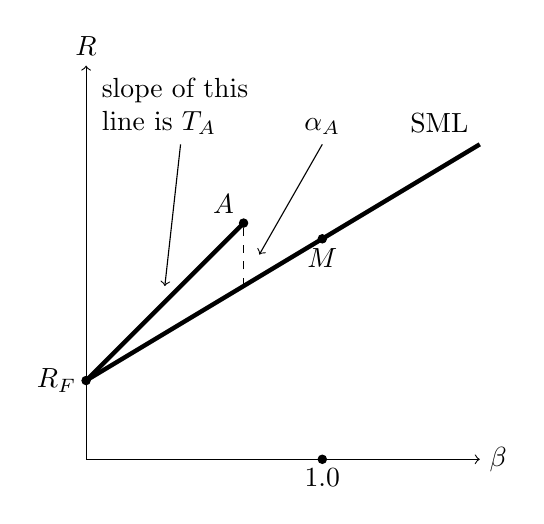
\begin{tikzpicture}
                \draw[->] (0, 0) -- (0, 5) node[above] {$R$};
                \draw[->] (0, 0) -- (5, 0) node[right] {$\beta$};
                \draw[ultra thick] (0, 1) -- (5, 4) node[above left] {SML};
                \draw[ultra thick] (0, 1) -- (2, 3);
                \draw[dashed] (2, 2.2) -- (2, 3);
                \draw[->] (3, 4) node[above] {$\alpha_A$} -- (2.2, 2.6);
                \draw[->] (1.2, 4) node[above, text width=2cm] {slope of this line is $T_A$} -- (1, 2.2);
                \draw[fill] (0, 1) circle[radius=1.5pt] node[left] {$R_F$};
                \draw[fill] (2, 3) circle[radius=1.5pt] node[above left] {$A$};
                \draw[fill] (3, 2.8) circle[radius=1.5pt] node[below] {$M$};
                \draw[fill] (3, 0) circle[radius=1.5pt] node[below] {1.0};
            \end{tikzpicture}
            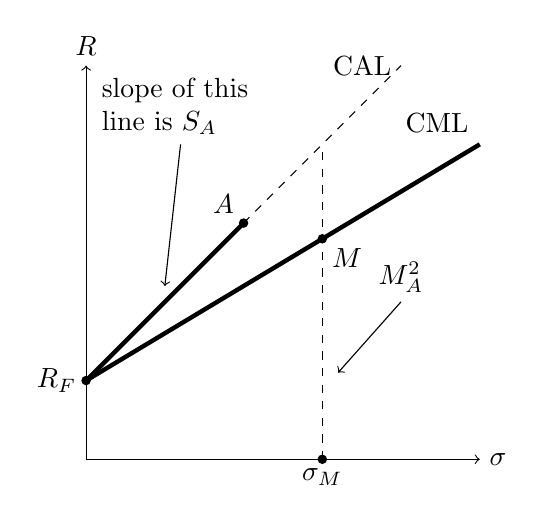
\begin{tikzpicture}
                \draw[->] (0, 0) -- (0, 5) node[above] {$R$};
                \draw[->] (0, 0) -- (5, 0) node[right] {$\sigma$};
                \draw[ultra thick] (0, 1) -- (5, 4) node[above left] {CML};
                \draw[ultra thick] (0, 1) -- (2, 3);
                \draw[dashed] (2, 3) -- (4, 5) node[left] {CAL};
                \draw[dashed] (3, 0) -- (3, 4);
                \draw[->] (4, 2) node[above] {$M^2_A$} -- (3.2, 1.1);
                \draw[->] (1.2, 4) node[above, text width=2cm] {slope of this line is $S_A$} -- (1, 2.2);
                \draw[fill] (0, 1) circle[radius=1.5pt] node[left] {$R_F$};
                \draw[fill] (2, 3) circle[radius=1.5pt] node[above left] {$A$};
                \draw[fill] (3, 2.8) circle[radius=1.5pt] node[below right] {$M$};
                \draw[fill] (3, 0) circle[radius=1.5pt] node[below] {$\sigma_M$};
            \end{tikzpicture}
        \end{center}
    \end{flushleft}
\end{flashcard}

\begin{flashcard}[\studyArea]{Considerations for Risk-Adjust Return Measures}
    \begin{itemize}
        \item Alpha and Treynor both use systematic risk. They agree in that positive alpha implies Treynor above the market. But they might not agree in relative ranking.
        \item Sharpe and $M^2$ both measure risk as total risk and higher Sharpe means higher $M^2$.
        \item Alpha and Treynor are criticized because they use beta and CAPM.
            \begin{itemize}
                \item Assumes single priced risk instead of multifactor model.
                \item Uses a market proxy, e.g.\ the S\&P 500 to stand for the market.
            \end{itemize}
        \item $M^2$ is criticized because the benchmark may not be replicable and transaction costs are not considered.
        \item Alpha, Treynor, and Sharpe are the more widely used measures.
        \item The highest relative return measure doesn't imply the highest actual return.
    \end{itemize}
\end{flashcard}

\begin{flashcard}[\studyArea]{Assumptions for Quality Control Charts}
    \begin{itemize}
        \item The null hypothesis states that the expected value-added return is zero.
        \item Value-added returns are independent and normally distributed.
        \item The investment process is consistent. The distribution of value-added returns is constant.
    \end{itemize}
\end{flashcard}

\begin{flashcard}[\studyArea]{Considerations and Policies for Manager Replacement}
    \begin{itemize}
        \item Assets in the existing manager's portfolio may have to be liquidated.
        \item Replacing a manager is requires time and effort from the fund sponsor.
        \item Replace managers only when justified. Short periods of underperformance are not justification.
        \item Develop formal policies and apply them to all managers.
        \item Use portfolio performance and other information for evaluation.
    \end{itemize}
\end{flashcard}

\begin{flashcard}[\studyArea]{Type I and Type II Errors}
    \begin{itemize}
        \item \textbf{Type I error} is rejecting the null hypothesis when it's true.
        \item \textbf{Type II error} is failing to reject the null hypothesis when it's false.
    \end{itemize}
\end{flashcard}
\end{document}
